% Created 2018-05-15 Tue 17:03
% Intended LaTeX compiler: pdflatex
\documentclass[11pt]{article}
\usepackage[utf8]{inputenc}
\usepackage[T1]{fontenc}
\usepackage{graphicx}
\usepackage{grffile}
\usepackage{longtable}
\usepackage{wrapfig}
\usepackage{rotating}
\usepackage[normalem]{ulem}
\usepackage{amsmath}
\usepackage{textcomp}
\usepackage{amssymb}
\usepackage{capt-of}
\usepackage{hyperref}
\usepackage[style=chicago-authordate,hyperref=true,backref=false,maxcitenames=3,url=false,eprint=false,doi=true,backend=biber,natbib=true] {biblatex}
\addbibresource{~/Dropbox/current_projects/RadicalOA-2018/Kelty-RP-OA.bib}
\usepackage{libertine}
\usepackage{libertinust1math}
\usepackage[T1]{fontenc}
\usepackage{setspace}
\author{Christopher Kelty}
\date{\today}
\title{}
\hypersetup{
 pdfauthor={Christopher Kelty},
 pdftitle={},
 pdfkeywords={},
 pdfsubject={},
 pdfcreator={Emacs 25.3.1 (Org mode 9.1.13)}, 
 pdflang={English}}
\begin{document}



\section*{Recursive Publics and Open Access (Version 1)}
\label{sec:org04d15e1}

\maketitle
\onehalfspacing 

Ten years ago, I published a book with Duke University Press called \href{https://twobits.net/download/index.html}{Two Bits: The Cultural Significance of Free Software} (\cite{kelty2008twobits}). The Press, and my editor Ken Wissoker, were enthusiastically accommodating of my demands to make the book freely and openly available.  Not only that, they also played along with my desire to release the ``source code'' of the book (i.e. HTML files of the chapters with minimal markup), and to compare the data on readers of the open version to buyers of the print.  It was a moment of exploration for both scholarly presses and for me. 

At the time, few authors were doing this other than Yochai Benkler (\cite{benkler2007wealnetw}) and \href{https://craphound.com/}{Cory Doctorow}, both of whom have also been activists and advocates for free software and open access, much as I have been.  We all shared, I think, a certain fanaticism of the convert that came from recognizing free software as an historically new, and radically different mode of organizing economic and political activity in Europe and America. \emph{Two Bits} gave me a way to talk not only about free software, but about open access and the politics of the university (\cite{kelty2008anthincirc,kelty2014beyoncopytech}).  It led me to engage in years of activism and writing on behalf of the ideas of open access and open science (see e.g. \href{https://osc.universityofcalifornia.edu/open-access-policy/policy-history/}{UC Open Access Policy}, \cite{kelty_outlaw_2010}) as well as the work I have done since then investigating participation (\cite{fish2011birdinter,kelty2018twomodespart}). 

Ten years later, I admit to a certain pessimism, if not outright depression at the way things have turned out.  Even barring the revelations of NSA spying, the destructive concentrated power of platform capitalism, and the proliferation of the worst forms of online hatred---the promise of free software has foundered, though it has not disappeared, and the question of what it means to achieve open access---or the goals of open access---has been swamped by concerns about costs, arcane details of repositories and versioning, and ritual offerings to the metrics God.  

When I wrote \emph{Two Bits}, it was obvious to me that the collectives who built free software were \emph{essential} to the very structure and operation of a standardized, singular Internet.  Free software and the Internet were related, as I said in the book, as figure and ground, by which I meant that they were indistinguishable until one focused on one or the other. Free software was the brain and the heart of the internet in the 1990s.  Today, free software is perhaps more like the blood of the internet: essential, but also more or less replaceable.

Today, free software and ``open source'' refer to quite dramatically different constellations of practice and people.  In 2006, I and many others saw little difference between these two names, and only Richard Stallman, in his characteristically fanatical way, insisted on the vapidity of the term ``open source''---though I followed his usage simply because I too cared more about freedom than openness.  But today, the two domains are in fact quite different.

Free software gathers around itself all those committed to the original and purist sense of a shared, collective, process of making software, tools, infrastructures, and hardware that cannot be appropriated by others, cannot be locked up, closed or otherwise sealed from the view anyone.  To this gravitational pull are attracted privacy and encryption advocates, certain kinds of legal advocates, activist hackers like LulzSec and Anonymous (\cite{coleman_hacker_2014}), and a subset of open access advocates who invested much effort in defining ``free culture'' on the very same rails as free software.  In political terms, I have always identified free software with a very specific, updated, version of classical Millian liberalism, warts and all.  It sustains a belief in the capacity for collective action and rational thought as aids to establishing a flourishing human livelihood.  But at the same time, it preserves an outdated blind faith in the automatic functioning of meritorious speech, a faith that the best ideas, given proper care and feeding, will inevitably rise to the top, regardless of context, situation, or history.  It is an updated classical liberalism that saw in software and networks a new place to resist the tyranny of the conventional and the taken for granted.  

By contrast, ``open source'' has come to mean something quite different: an ecosystem controlled by an oligopoly of firms which maintains a shared pool of components and frameworks that lower the costs of education, training, and software creation in the service of establishing winner-take-all platforms.  Winner-take-all platforms are built on open source, but they do not carry the principles of freedom or openness all the way through to the platforms themselves (cf. \href{https://platform.coop/directory}{platform cooperativism}).  What open source has become is now almost the opposite of free software:  a way of subordinating the tools and infrastructures needed for any kind of collective activity to the dominance of a handful of platform companies whose platforms are parasitic on the very tools and infrastructures designed to support them---it is authoritarian, plutocratic, and nepotistic, everything liberalism wanted to resist. Also, \$. 

Inertia and capital have taken control---not so much of the means of production, nor the products themselves---of the very content of work.   For example, when we talk about things like precarious labor and platforms such as Uber or Task Rabbit, it is clear that the software and infrastructures they are built upon rely on the fruits of the labor of ``open source'' (whether that be the programming languages or the operating systems or higher-level frameworks); however, the platforms that result do not follow the same principles---they are not open or free in any meaningful sense.  Quite the reverse: their profitability demands that the labor of open source and free software creators is more often directed towards improvements in the underlying infrastructure which serve these platforms---and not the interests of the programmers, engineers, designers, or users who must maintain them, or live by them on a daily basis--- to say nothing of the Uber drivers or task rabbits who live by the platforms.  What  matter open source if the software and tools are only of use to a handful of giant corporations?  What matter free software if freedom is only in the service of someone else's fiefdom and worldview. 

Does open access face the same problem?  In 2007, when I imagined applying the principles of Free Software to my own book---it was not simply a question of making the book openly accessible.  It was instead an attempt to think about the tools and infrastructures at the heart of productive, collective scholarly work and labor.  What makes a book good? How do people learn from it, re-use it, extend it, critique it?  And how do we keep track of that? What ``memory practices'' do we use (\cite{bowker2005memorpracscien}), and how should they be transferred to the milieu of digital, networked environment?

In part my desire to ``free the source'' of my book grew out of the unfinished business of digitizing the scholarly record and the library.  To my mind, the archival functions of the library---preservation, metadata, cataloging, findability, etc---were not adequately reproduced in the wilds of the 2006-7 Internet, despite incredibly powerful tools for doing so. The importance of these functions is not marginal or trivial---it is the very substance of the \emph{community} of scholarship, it is what allows scholarship to accumulate collectively and in common, rather than as the private ownership of select individuals. The \emph{infrastructure} of scholarship is not an afterthought, but a \emph{sine qua non}.  Critique requires memory practices that are shared amongst a community of scholars---or else it becomes an idle pursuit of the few. 

Indeed, it is an irony that much of the work that went into designing the internet at its outset in the 1980s, such as gopher, WAIS, and the HTML of CERN, was conducted in the name of the digital transformation of the library.  But by 2007, these aims were swamped by attempts to transform the Internet into a giant factory of data extraction, and wars over winner-take-all platforms for spying and surveillance in the name of advertising dollars.  Even in 2006-7 it was clear that this unfinished business of digitizing the scholarly record was going to become a problem---both because it was being overshadowed by other concerns, and because of the danger it would eventually be subjected to the very platformization underway in other realms. 

\begin{figure}[htbp]
\centering
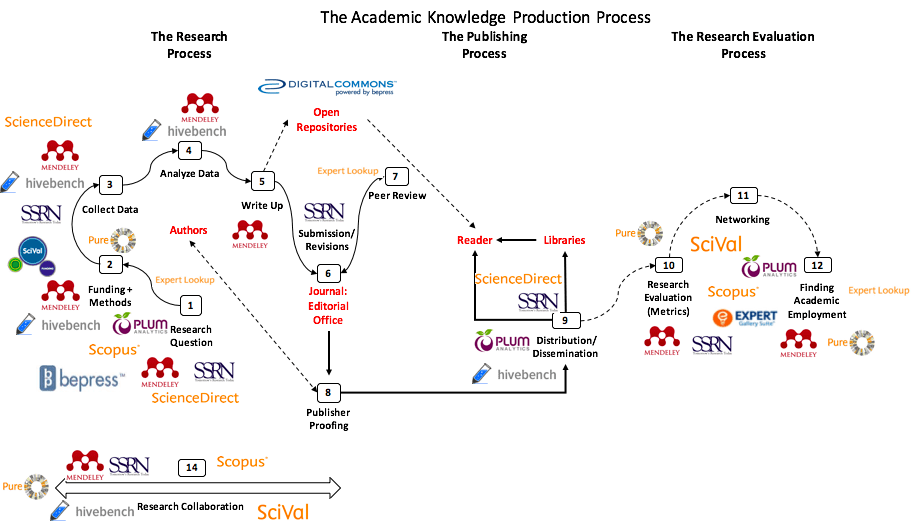
\includegraphics[width=.9\linewidth]{./with-companies.png}
\caption{\label{fig:orgea685dc}
From ``\href{http://knowledgegap.org/index.php/sub-projects/rent-seeking-and-financialization-of-the-academic-publishing-industry/preliminary-findings/}{Rent Seeking by Elsevier}.'' by Alejandro Posada and George Chen (Showing all of the companies along the pipeline owned by Elsevier).}
\end{figure}


Because if the platform capitalism of today has ended up being parasitic on the free software tools and infrastructures that enabled it, then why would this not also be true of science and scholarship more generally?  Are we not witnessing a transition to a world where science and scholarship are directed---in their very content and organization---towards the profitability of the platforms that ostensibly serve it? (See, e.g. Figure 1 from \href{http://knowledgegap.org/index.php/sub-projects/rent-seeking-and-financialization-of-the-academic-publishing-industry/preliminary-findings/}{this post})  Is it not possible, that the platforms created to ``serve science'' ---Elsevier's increasing acquisition of tools to control the entire life-cycle of research, or ResearchGate's ambition to become the single source for all academics to network and share research---that these platforms might actually end up warping the very content of scientific and scholarly production in the service of their profitability?  Perhaps we are too late?  If we wonder, today, why science seems to have so little effect on the world around us, perhaps it is because it has forsaken its duty to govern itself?

To put this even more clearly: open access has come to exist and scholarship is more available and more widely distributed than ever before in history.  But, scholars now have less control, and have taken less responsibility for the means of production of scientific research, it's circulation, and perhaps even the content of that science.  

\subsection*{The Method of Modulation}
\label{sec:org2ab459a}

Although I have been an activist for open access, I remain fundamentally a scholar, with only the meager skills that implies. As such, I think there may yet me something to learn about the ways that open access has unfolded in the last decade, and the problems we face now, and that this kind of careful critique still has a role to play (\cite{foucault1997critique,folkers2015darintrut}).  When I wrote \emph{Two Bits} I organized the argument around the idea of \emph{modulation}: free software is simply one important assemblage of technologies, practices, and people aimed at resolving certain problems of the relationship of knowledge (or software tools related to knowledge) and power (\cite{hacking2004histontol,rabinow2003anthtoday}).  One can still, I think, observe how these different elements have in been taken up and worked over as part of what we now identify as the problem of open access---as well as the arrival of other elements that were not part of free software---in order to track this modulation and its direction, sedimentation, or dispersal.

\subsubsection*{\textbf{sharing source code}:}
\label{sec:org62dfbf7}
Shareable source code was a concrete and necessary achievement for Free Software to be possible.  Similarly, the necessary ability to share and circulate digital texts is a significant achievement---but such texts are shareable in a much different way.  For source code, computable streams of text are everything---anything else is a ``blob'' like an image, a video or any binary file. But scholarly texts are, with rare exceptions, blobs: Word or Portable Document Format (PDF) files.   What's more, while software programmers may love ``source code'', academics generally hate it--- anything less than the final, typeset version of a text is considered something unfinished (see e.g. the endless disputes over ``author's final versions'' that plague open access debates; see \href{http://www.sherpa.ac.uk/romeo/index.php}{Sherpa/ROMEO}).  Finality is important to scholarship.  Modifiability of a text, especially in the humanities and social sciences, is acceptable only when it is an experiment of some kind.

What's shared, then, is less a tool or a substrate or a ``source'' and more a product: results, findings, abstracts, titles, \emph{products}.   The real source code is not the digital text, it is the ideas, arguments, findings etc.  (cf. \href{https://en.wikipedia.org/wiki/Least\_publishable\_unit}{The Least Publishable Unit} or the Journal \emph{\href{https://www.sciencematters.io/why-matters}{Science Matters}}).  In an sense, the source code of science is not a code at all, but a more abstract set of relations between concepts, theories, tools, methods, and the disciplines and networks of people who operate with them, critique them, extend them and try to maintain control over them even as they are shared within these communities.  I wrote about this ``constitutive closure'' of science in an \href{https://kelty.org/or/papers/Kelty-biosoc20128a.pdf}{article} on genetics in the 1930s (\cite{kelty2012not}).

\subsubsection*{\textbf{defining openness}:}
\label{sec:org1a4eb13}

In order for Free Software to make sense as a solution, those involved first had to characterize the problem it solved---and they did so by identifying a pathology in the worlds of corporate capitalism and engineering in the 1980s: that computer corporations were closed organizations who re-invented basic tools and infrastructures in a race to dominate a market.    An ``open system,'' by contrast, would avoid the waste of ``reinventing the wheel'' and of pathological competition, allowing instead  modular, reusable parts that could be modified and recombined to build better things in an upward spiral of innovation.  The 1980s ideas of modularity, modifiability, abstraction barriers, interchangeable units have been essential to the creation of the digital infrastructures we live with, and form the basis for waves of innovation that occur just below the threshold of mass public visibility, but which are obvious to engineers and software coders in the industry. 

To propose an ``open science'' thus modulates this definition---and the idea works in some sciences better than others.  Aside from the obviously different commercial contexts, philosophers and literary theorists just don't think about openness this way--- theories and arguments may be used as building blocks, but they are not modular in quite the same way.  Indeed, it is essential that they remain tied to the individuals who uttered them---concepts are owned and sacred.  Molecular biologists, to take a contrasting example make advances precisely through all kinds of re-combinations of material components and theories in a lab, much of which then form the basis for advances in pharma, ag, and biotech.    In either case though, the free circulation of the work whether for recombination, or for reference and critique, remains a \emph{sine qua non} of the theory of openness proposed there.   It is opposed to a system where it is explicit that only certain people have access to the texts (whether that be through limitations of secrecy, or limitations on intellectual property--- though it can be one that is implicitly restricted to those who are elites, have paid, or otherwise are ``in the know'').  Different disciplines seem to be made more or less uncomfortable by openness.  In mathematics, for instance, the idea is anathema that a worthy proof might be ignored or lost because its author is not elite, not allowed access to a publication (either to read or to publish in) or is in any other way prevented from making his or her solution known. Whereas, in art history, reputation, networks, and style often count as much as content. 

\subsubsection*{\textbf{Writing and using copyright licenses}.}
\label{sec:org6bed922}

Of all the components of free software that I analyzed, this is the one practice that remains the least transformed--- open access texts use the same CC licenses that I watched  Boyle and Lessig pioneer in 2001, which were a direct result of their engagement with free software licenses.

A novel modulation of these licenses is the \textbf{open access policies} pioneered in other ways and places as part of the development of OA (the embrace of OA in Brazil for instance, or the spread of OA Policies starting with Harvard and the University of California's activism around them in 2008).  Today the ability to control the circulation of a text with IP rights is far less economically central to the strategies of publishers than it was in 2007, even if they persist in attempting to do so\ldots{} they have loosened author agreements and allowed circulation in ways that are far less restrictive.  At the same time, funders, states, and universities have all adopted patchwork policies intended to both sustain green OA, and push publishers to innovate their own business models in gold and hybrid OA.  While ``Green OA'' is a significant success on paper, the actual use of it to circulate work pales in comparison to the commercial control of circulation on the one hand, and the increasing success of shadow libraries on the other. Repositories have sprung up in every shape and form, but they remain largely \emph{ad hoc}, poorly coordinated, and underfunded solutions to the problem of OA.

\subsubsection*{\textbf{coordinating collaborations}.}
\label{sec:org6c85a56}

The \emph{collective} activity of Free Software is ultimately the most significant of its achievements---marrying a form of intensive small-scale interaction amongst programmers, with sophisticated software for managing complex objects (version control and GitHub-like sites).  There has been constant innovation in these tools for controlling, measuring, testing, and maintaining software.

By contrast, the collective activity of scholarship is still largely a pre-modern affair.  It is coordinated largely by the idea of ``writing an article together'' and not by working to maintain some larger map of what a research topic, community, or discipline has explored--- what has worked and what has not. 

This is--to some extent, what I sought to do by ``freeing the source code'' to my book.  Indeed, when I wrote to Duke University Press to suggest the idea, I tried to articulate this, by contrast with a very similar attempt by Yochai Benkler.  He had created a wiki-fied version of his book \emph{The Wealth of Networks} (\cite{benkler2007wealnetw}) and invited anyone to update or improve it.  In contrast to an encyclopedia article, I argued, a scholarly book or article is a much different kind of thing:  if people are to collaborate, they demand to be involved much earlier in the process, or they want to take bits and pieces of the argument and write \emph{their own articles and books}.  Nonetheless it seemed to me that a system--- even just a system of websites, blogs, and repositories focused on a topic was a necessary innovation at the time. 

This focus on the coordination of collaboration seemed to me to be one of the key advantages of free software, but it has turned out to be almost totally absent from the practice or discussion of open access.  Collaboration and the recombination of elements of scholarly practice obviously happens, but it does not depend on open access in any systematic way: there is only the counterfactual that without it, many different kinds of people are excluded from collaboration or even simple participation in, science and scholarship, something that most active scholars are willfully ignorant of.

But the major publishing companies as well as open science advocates get this: and they have turned towards establishing work-flow tools and frameworks---of varying flexibilities---that are intended to fill this gap.  Elsevier has explicitly begun to think about its role as a provider of such frameworks, while other more cooperative projects like Humanities Commons or the shadow libraries (Monoskop, Memory of the World, Aaaaarg.org) have offered different kinds of alternative spaces for coordinating collaboration.

\subsubsection*{\textbf{Fomenting a movement}:}
\label{sec:orgb17e2c5}

I demoted the idea of a social movement to merely one component of the success of free software, rather than let it be---as most social scientists would have it---the principal container for free software.  As important as movements and their participants are, they are not the whole story, but only part of it.  

Is there an open access movement?  Yes and no.  Librarians remain the most activist and organized of the bunch.  The handful of academics who care about it have shifted to caring about it in primarily a bureaucratic sense, forsaking the cross-organizational aspects of a movement in favor of activism within universities (to which I plead guilty, and which is hard enough as it is).  But this transformation forsakes the need for addressing the collective, collaborative responsibility for scholarship in favor of letting individual academics, departments, and disciplines be the focus for such debates. 

By contrast, the publishing industry works with a phantasmatic idea of both an open access ``movement'' and of the actual practices of science and scholarship--- they too defer, in speech if not in practice, to the academics themselves, but at the same time must create tools, innovate processes, establish procedures, acquire tools and companies an so on in an effort to capture these phantasms and to prevent academics from collectively doing so on their own. 


\textbf{And what new components?}  The five above were central to Free Software as I analyzed it up to about 2006.  But open access has other components that are arguably more important to its organization and transformation.

\subsubsection*{\textbf{Money, i.e. Library Budgets}:}
\label{sec:orgb2afcbe}
Central to almost all of the politics and debates about open access is the political economy of publication.  From the ``bundles'' debates of the 1990s to the gold/green debates of the 2010s, the sole source of money for publication long ago shifted into the library budget. The relationship that library budgets have to other parts of the political economy of research (funding for research itself, debates about tenured/non-tenured, adjunct and other temporary salary structures) has shifted as a result of the demand for open access, leading libraries to re-conceptualize themselves as potential publishers, and publishers to re-conceptualize themselves as serving a ``life cycles'' or ``pipeline'' of research, not just its dissemination.

\subsubsection*{\textbf{Metrics}}
\label{sec:org23ae73d}
More than anything, Open Access is promoted as a way to continue to feed the metrics gods.  OA means more citations, more easily computable data, and more visible uses and re-uses of publications (as well as ``open data'' itself, when conceived of as product and not measure).  The innovations in the world of metrics---from the quiet expansion of the platforms of the publishers, to the invention of ``alt metrics'' to the enthusiasm of ``open science'' for metrics-driven scientific methods, this component forms a core feature of what ``open access'' is today, in a way that was not true of Free Software before it (in that case-- users, downloads, commits, lines of code were always after-the-fact measures of quality, and not constitutive ones).  

Other components of this sort might be proposed in an historical-ontological analysis of the transformation of open access, but the main point of an exercise like this is to resist the temptation to clutch open access as if it were the beating heart of a social transformation in science, as if it were  \emph{thing} that must exist, rather than a configuration of elements at a moment in time.  Open Access was a solution---but it is too easy to lose sight of the problem. 

\subsection*{Open Access without Recursive Publics}
\label{sec:orgf11f1a0}

When we no longer have any commons, but only platforms, will we any longer have knowledge as we know it?  This is a question at the heart of research in the philosophy and sociology of knowledge---not just a concern for activism or social movements.  If knowledge is socially produced and maintained, then the nature of the social bond surely matters to the nature of that knowledge.   This is not so different than asking whether we  will still have labor or work, as we have long known it, in an age of precarity?  What is the knowledge equivalent of precarity (i.e. not just the existence of precarious knowledge workers, but a kind of \emph{precarious knowledge} as such)?  Do we not already see the evidence of this in the ``post-truth'' of fake news, the deliberate and aggressive refusal to believe in evidence, truth, established systems of argument and debate, the very capacity to establish critique as a line along which one travels towards values like justice or equality?

I think the relationship between knowledge and power is shifting dramatically, because the costs---and the stakes---of producing high quality, authoritative knowledge have also shifted.  It is not so powerful any longer; science does not speak truth to power because truth is no longer so obviously important to power---and this is a mystery to me and many other people.  It is not the case that expertise and the production of quality science, good numbers, and clear arguments are irrelevant---they still hold a central place in the world, but they do not function in just the way we might expect them to when we talk about the virtues of open access, circulation or sharing.  It may be the case that science no longer stands outside power as it once did, but works through it ever more diligently and silently.

Although this is a pessimistic portrait, it may also be a sign of something yet to come.  Free Software as a community, has been and still sometimes is critiqued as being, to put it bluntly, an exclusionary space of white male sociality (\cite{nafus_patches_2012,massanari2016fapp,ford2017canedit,reagle2013freeassexis}).  I think this critique is true, but it is less a problem of identity than it is a pathology of a certain form of liberalism: a form that demands that merit consists only in the \emph{content} of the things we say (whether in a political argument, a scientific paper, or a piece of code), and not in the ways we say them, or who is encouraged to say them and who is encouraged to remain silent (\cite{dunbar-hester_low_2014}).

One might, as a result, choose to throw out liberalism altogether as a broken philosophy of governance and liberation.  But it might also be an opportunity to focus much more specifically on a particular problem of liberalism, one that the discourse or open access also relies on to a large extent.  Perhaps it is not the case that merit derives solely from the content of utterances freely and openly circulated, but also from the \emph{ways in which they are uttered, and the dignity of the people who utter them}.  An open access (or a free software) that embraced that principle would demand that we pay attention to different problems:  how are our platforms, infrastructures, tools organized and built to support not just the circulation of putatively true statements, but the ability to say them in situated and particular ways, with respect for the dignity of who is saying them, and with the freedom to explore the limits of \emph{that} kind of liberalism, should we be so lucky to achieve it. 

\printbibliography
\end{document}